\documentclass[12pt, twoside]{book}
%\documentclass[12pt, oneside]{book}  % jednostranna tlac

% spravne nastavenie okrajov
\usepackage[a4paper,top=2.5cm,bottom=2.5cm,left=3.5cm,right=2cm]{geometry}
% zapnutie fontov pre UTF8 kodovanie
\usepackage[utf8]{inputenc}
\usepackage[T1]{fontenc}

% nastavenie riadkovania podla smernice
\linespread{1.25} % hodnota 1.25 by mala zodpovedat 1.5 riadkovaniu

% balicek pre lepsie zobrazovanie referencii
\usepackage[backend=biber]{biblatex}
\addbibresource{references.bib}

% pridanie balicku pre pokrocile pouzivanie farieb
\usepackage{xcolor}

% definovanie farby pozadia pre command-line
\definecolor{background}{rgb}{0.95,0.95,0.95}
\definecolor{placeholder}{rgb}{0.07,0.04,0.56}
\definecolor{string}{rgb}{0.0,0.5,0.0}
\definecolor{highlight}{rgb}{0.8,0.0,0.0}
\definecolor{comment}{rgb}{0.66, 0.66, 0.66}

% balicek na vkladanie obrazkov
\usepackage{graphicx}

% balicek na vkladanie celych pdf dokumentov, tu zadanie
\usepackage{pdfpages}

% balicek na spravne formatovanie URL
\usepackage{url}
% balicek na hyperlinky v ramci dokumentu
% zrusime farebne ramiky okolo liniek aby pdf
% vyzeralo rovnako ako tlacena verzia
\usepackage[hidelinks,breaklinks]{hyperref}

% balicek pre oramovanie command-line-u
\usepackage{mdframed}

% idk
\usepackage{fancyvrb}

% balicek na vkladanie zdrojoveho kodu
\usepackage{listings}

% definovanie prikazu pre TODO poznamku
\newcommand{\TODO}[1]{\textcolor{blue}{TODO -- #1}}

\newcommand{\shell}{\textcolor{placeholder}{<SHELL>}}
\newcommand{\host}{\textcolor{placeholder}{<HOST>}}
\newcommand{\port}{\textcolor{placeholder}{<PORT>}}
\newcommand{\portt}{\textcolor{placeholder}{<PORT2>}}
\newcommand{\file}{\textcolor{placeholder}{<FILE>}}

\newenvironment{cmdframe}
	{\begin{mdframed}[
	backgroundcolor=background,
	linecolor=black,
	roundcorner=10pt,
	innerleftmargin=10pt,
	innerrightmargin=10pt,
	innertopmargin=5pt,
	innerbottommargin=5pt
	]}
	{\end{mdframed}}
    
\newenvironment{cmdline}[4]
{\begingroup\lstset{
	language={#1},
	otherkeywords={#3},
	morekeywords=[1]{#3},
	morekeywords=[2]{#4},
	basicstyle={\ttfamily\footnotesize},
	backgroundcolor={\color{background}},
	commentstyle={\color{comment}},
	stringstyle={\color{string}},
	keywordstyle={\color{highlight}},
	keywordstyle=[2]{\color{blue}},
	showspaces=false,
	showstringspaces=false,
	columns=fullflexible,
	breaklines=true,
	escapechar={#2}
}\VerbatimOut{tmp.txt}}
{\endVerbatimOut\begin{cmdframe}\lstinputlisting{tmp.txt}\end{cmdframe}\endgroup}

\newcommand{\dpd}[1]{\textbf{Dependencies:} #1}

\newcommand{\notte}[1]{\small \textbf{Note:} #1}

% -------------------
% --- Definicia zakladnych pojmov
% --- Vyplnte podla vasho zadania, rok ma byt rok odovzdania
% -------------------
\def\mfrok{2024}
\def\mfnazov{Analysis of reverse shell techniques and possible countermeasures}
\def\mftyp{Bachelor Thesis}
\def\mfautor{Matúš Bucher}
\def\mfskolitel{Ing. Dušan Bernát, PhD.}

\def\mfmiesto{Bratislava, \mfrok}

\def\mfodbor{Computer Science}
\def\program{Computer Science }

\def\mfpracovisko{ Department of Computer Science }

\begin{document}     
\frontmatter
\pagestyle{empty}

% -------------------
% --- Obalka ------
% -------------------

\begin{center}
  \sc\large
  Comenius University in Bratislava\\
  Faculty of Mathematics, Physics and Informatics

\vfill

{\LARGE\mfnazov}\\
\mftyp
\end{center}

\vfill

{\sc\large 
\noindent \mfrok\\
\mfautor
}

\cleardoublepage
% --- koniec obalky ----

% -------------------
% --- Titulný list
% -------------------

\noindent

\begin{center}
\sc  
\large
  Comenius University in Bratislava\\
  Faculty of Mathematics, Physics and Informatics

\vfill

{\LARGE\mfnazov}\\
\mftyp
\end{center}

\vfill

\noindent
\begin{tabular}{ll}
Study Programme: & \program \\
Field of Study: & \mfodbor \\
Department: & \mfpracovisko \\
Supervisor: & \mfskolitel \\
\end{tabular}

\vfill


\noindent \mfmiesto\\
\mfautor

\cleardoublepage
% --- Koniec titulnej strany


% -------------------
% --- Zadanie z AIS
% -------------------
% v tlačenej verzii s podpismi zainteresovaných osôb.
% v elektronickej verzii sa zverejňuje zadanie bez podpisov
% v pracach v anglictine anglicke aj slovenske zadanie

\newpage
\setcounter{page}{3}
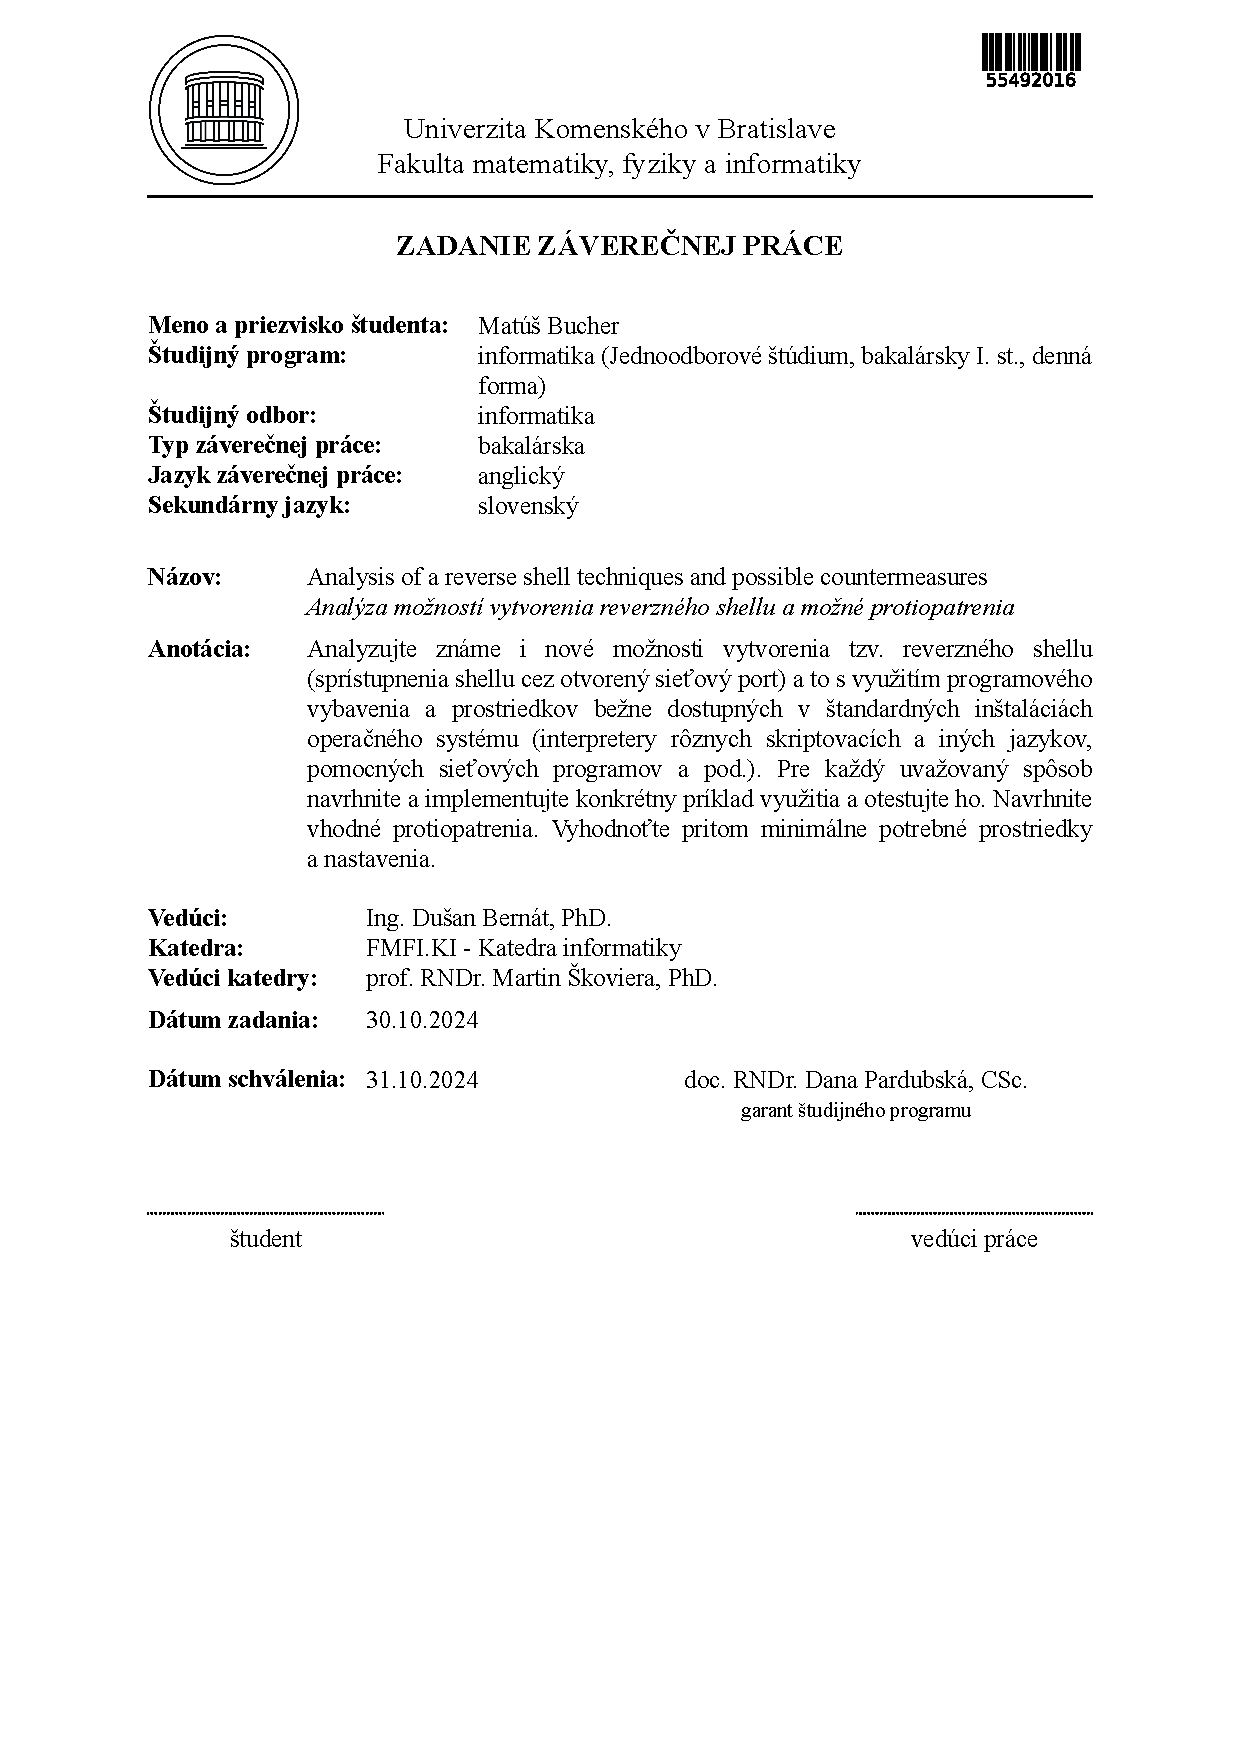
\includepdf{images/zadanie.pdf}

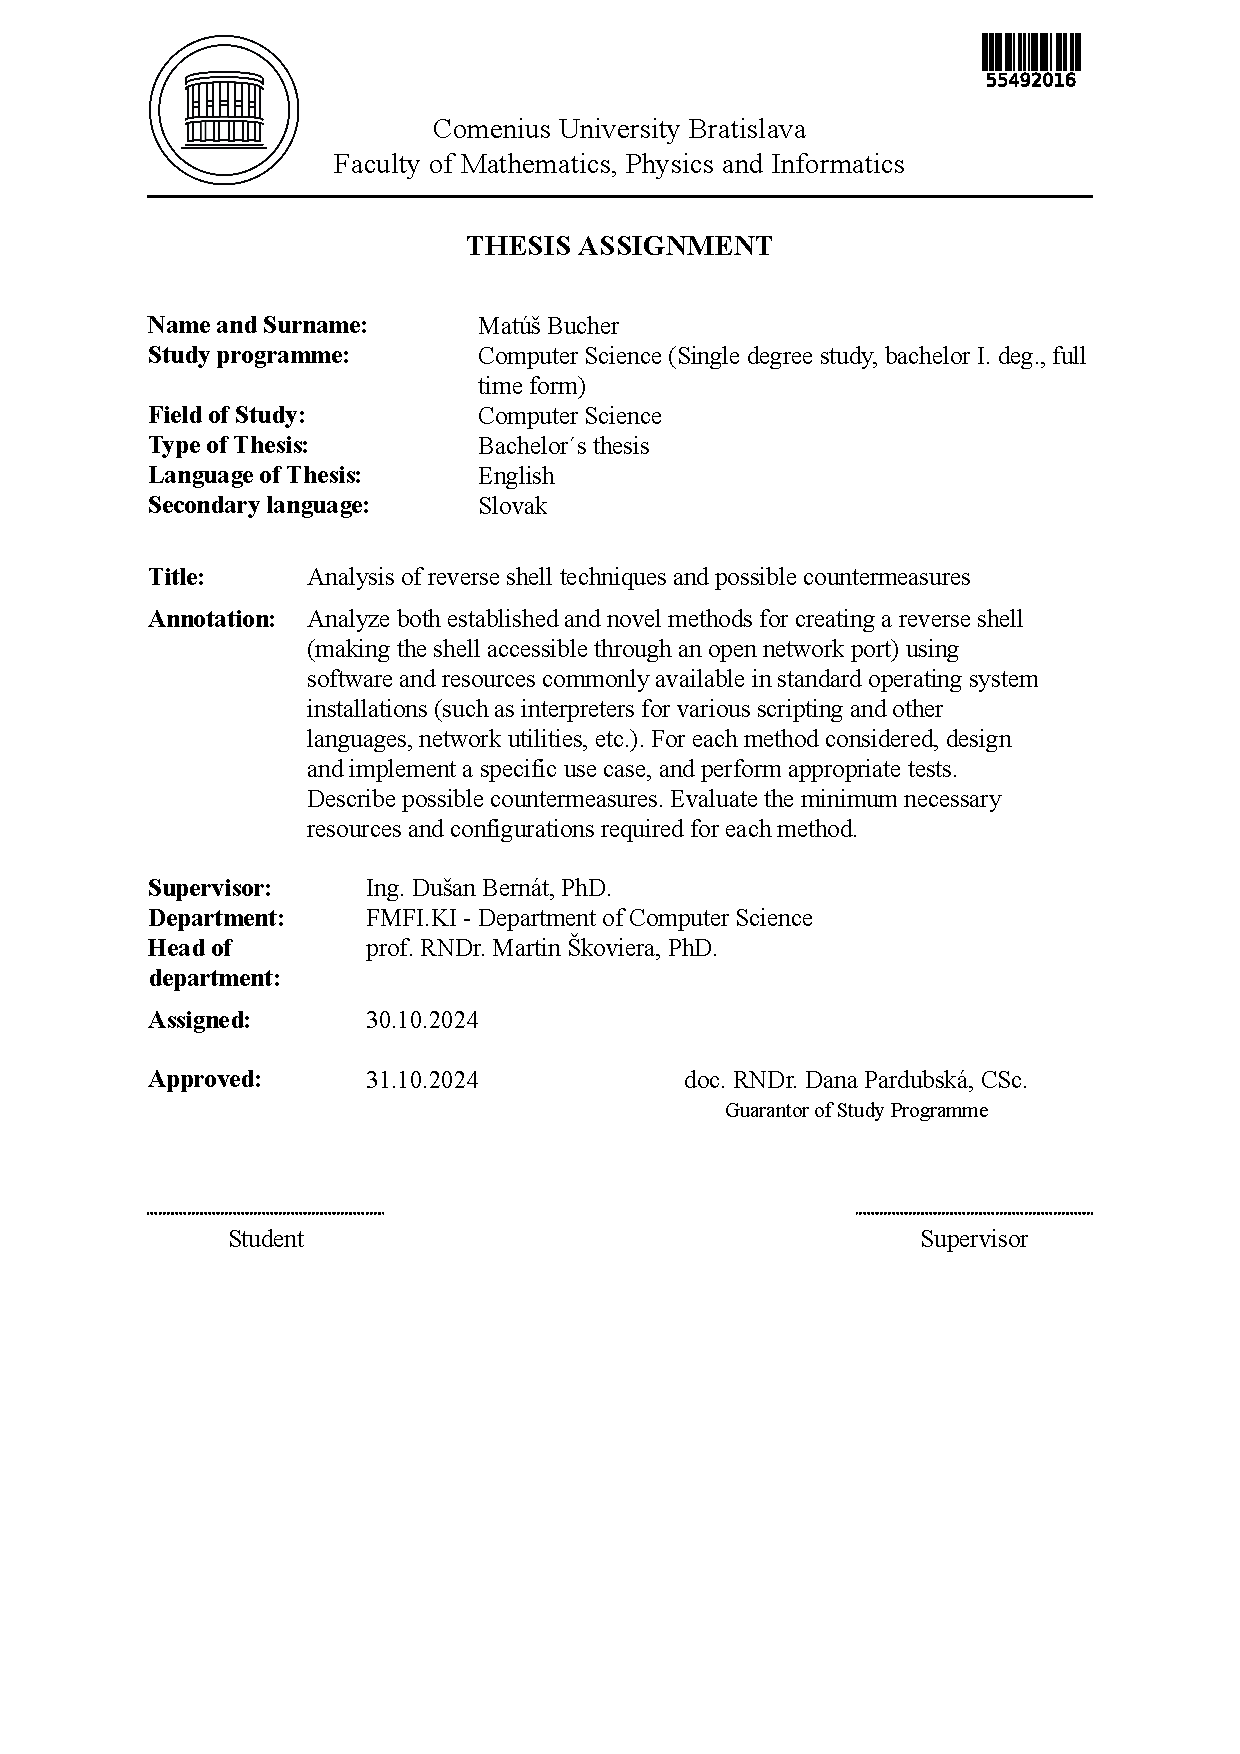
\includepdf{images/zadanie-en.pdf}

% --- Koniec zadania


% -------------------
%   Poďakovanie - nepovinné
% -------------------
\newpage
\pagestyle{plain}
~

\vfill
{\bf Acknowledgments:} \TODO{add acknowledgments}

% --- Koniec poďakovania

% -------------------
%   Abstrakt - Slovensky
% -------------------
\newpage 
\section*{Abstrakt}


\TODO{add abstract in Slovak}

\paragraph*{Kľúčové slová:} \TODO{add keywords in Slovak}
% --- Koniec Abstrakt - Slovensky


% -------------------
% --- Abstrakt - Anglicky 
% -------------------
\newpage 
\section*{Abstract}

\TODO{add abstract in English}


\paragraph*{Keywords:} \TODO{add keywords in English}

% --- Koniec Abstrakt - Anglicky

% -------------------
% --- Predhovor - v informatike sa zvacsa nepouziva
% -------------------
%\newpage 
%
%
%\chapter*{Preface} %
%
%Predhovor je všeobecná informácia o práci, obsahuje hlavnú charakteristiku práce 
%a okolnosti jej vzniku. Autor zdôvodní výber témy, stručne informuje o cieľoch 
%a význame práce, spomenie domáci a zahraničný kontext, komu je práca určená, 
%použité metódy, stav poznania; autor stručne charakterizuje svoj prístup a svoje
%hľadisko. 
%
% --- Koniec Predhovor


% -------------------
% --- Obsah
% -------------------

\cleardoublepage 

\tableofcontents

% ---  Koniec Obsahu

% -------------------
% --- Zoznamy tabuliek, obrázkov - nepovinne
% -------------------

\newpage 

\listoffigures
\listoftables

% ---  Koniec Zoznamov

\mainmatter
\pagestyle{headings}

\input intro.tex 

\input chapters/chapter00.tex

\input chapters/chapter01.tex

\input chapters/chapter02.tex

\input chapters/chapter03.tex

\input conclusion.tex



%\input zaver.tex

% -------------------
% --- Bibliografia
% -------------------


\newpage	

\backmatter

\thispagestyle{empty}
\clearpage

\printbibliography 

%---koniec Referencii

% -------------------
%--- Prilohy---
% -------------------

%\input appendixA.tex

%\input appendixB.tex

\end{document}
